
\newcommand{\BF}{\mathbf{F}}
\newcommand{\BZ}{\mathbf{Z}}
\newcommand{\BA}{\mathbf{A}}
\newcommand{\BB}{\mathbf{B}}
\newcommand{\BC}{\mathbf{C}}
\newcommand{\BD}{\mathbf{D}}

A pilot study aims at examining how humans learn compliant force dynamics and
modulate their whole-body motions to reach anticipated goals.  Here, we
present an experimental idea to measure the goal-directed movements against
compliant forces, and then illustrate the ongoing results which were conducted
for a few human subjects.  At this pilot stage, we are focusing on the simple
linear compliant case and discuss further experiments.  To deepen
understanding of the mechanism in humans, it would be beneficial to develop
the humanoid robot control in interacting with multiple compliant surfaces.

%%%%%%%%%%%%%%%%%%%%%%%%%%%%%%%%%%%%%%%%%%%%%%%%%%%%%%%%%%%%%%%%%%%%%%%%%%%%%%%%
\section{Introduction}

Humans can learn how to control their own body movements in an uncertain
environment, and utilise it to predict the consequences of actions and to
achieve a behavioural goal \cite{Wolpert11, Davidson&Wolpert03}.  A
considerable amount of research has shown the human capabilities of
generalization in visuomotor learning and has been exploring the underlying
mechanisms \cite{Goodbody&Wolpert98, Krakauer06}.  A certain exposure to a new
physical environment facilitates to generalize the spatial and temporal
characteristics of the point-to-point movements via error-based learning and
perturbation paradigm. In the real-world interactions, there are varied and
complicated force dynamics (i.e., governed by not only simple linear
principles) when making a contact with an object and handling it. The optimal
functions seem to be perceptually learned via repetitive movements against the
force. However, to our knowledge, little is still known about how humans can
generalize the compliant force dynamics itself and utilize it to their future
motor plan.

The CoDyCo project has been investigating the whole-body coordination
mechanisms in arm reaching movements and the postural balance control in
assistive contact with rigid and/or compliant surfaces. Like humans, robots
are required to flexibly adjust their posture and to coordinate the physical
mobility with augmented autonomy. We expect that humans could generalize the
force principles in a cognitively robust way via force-feedback from the early
stage of the body movements. To explore the generalization mechanism of the
force dynamics in humans and to model it would provide a useful strategy in
humanoid robot control. The successful model could be exploited to effectively
control autonomous robots' whole-body balance in interacting with the
environment through supportive contacts.

In a pilot study, we focused on a simple case: linear compliant force. 
We employed a haptic device, Haptic Master (Moog, Inc.), which is controlled by 
a set of a computer programmes to render robotic manipulandum for force 
feedback. The pilot experiment measured the end-effector movements controlled 
by human subjects and analysed the dynamic properties of the movements against 
the compliant force and the performance.


%%%%%%%%%%%%%%%%%%%%%%%%%%%%%%%%%%%%%%%%%%%%%%%%%%%%%%%%%%%%%%%%%%%%%%%%%%%%%%%%
\section{Methods}

\subsection{Modelling}

In general, spring-damper force ($\BF$) is formulated by the position and the
velocity with parameters: spring stiffness ($k$) and spring damping factor
($\lambda$).  Here, it is simplified for one direction ($\BZ$).
%
\begin{equation}
  \BF = k \BZ^n + (\lambda \BZ^p) \dot{\BZ} \, .
\end{equation}
%

We employed the ready-made spring model in the Haptic API, where the 
compliant force formula was assigned to the device, the Haptic Master. 
The compliant force was rendered by the end-effector position and the 
velocity with the parameters in real-time (Fig. 1). 
%
\begin{figure}
  \centering
  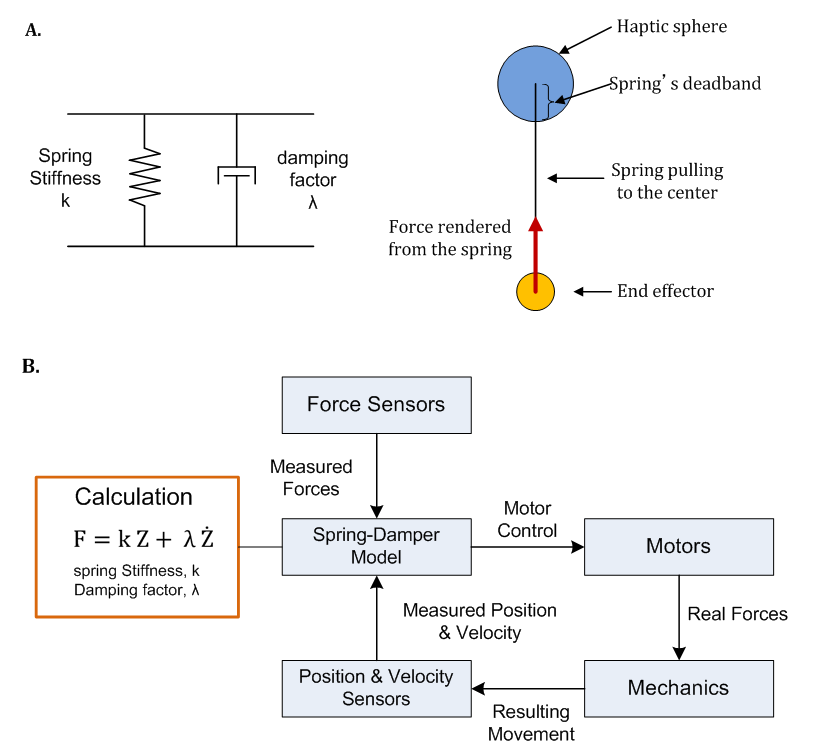
\includegraphics[scale=0.5]{Chie/figs/fig1.png}
  \caption{A. The ready-made spring model in the Haptic API. B. Block 
   diagram of the compliant force control. The force is rendering
   based on the end-effector position and the velocity with parameters 
   (spring stiffness and damping factors) in the real time.}
  \label{modelling}
\end{figure}


\subsection{Experimental Design}

As a pilot study, we employed a simple linear spring-damper formula:
%
\begin{equation}
  \BF = k \BZ + \lambda \dot{\BZ} \, .
\end{equation}
%
The compliant force formula is assigned to the model in the Haptic
Master. Aiming to simplify analysing the performance, the forces and the
movements were constrained in the only one direction, here, in the vertical
(Z) direction to the ground.

Human subjects learned a spring compliant force via repetitive reaching
Bmovements to the first target (z = t1) in a certain period of time, - so
called ``Learning session''.  Then, they were asked to move the end-effector
to the second, or test, target (z = t2), which was set more far from the t1
position, as a test trial; so, more force would be required for this movement
(Fig.2). In order to achieve the t2 target, the participants would exploit
their prior knowledge of the force dynamics experienced via learning
session. We will evaluate whether and how the motion performance is likely to
follow the formula previously learned.
%
\begin{figure}
  \centering
  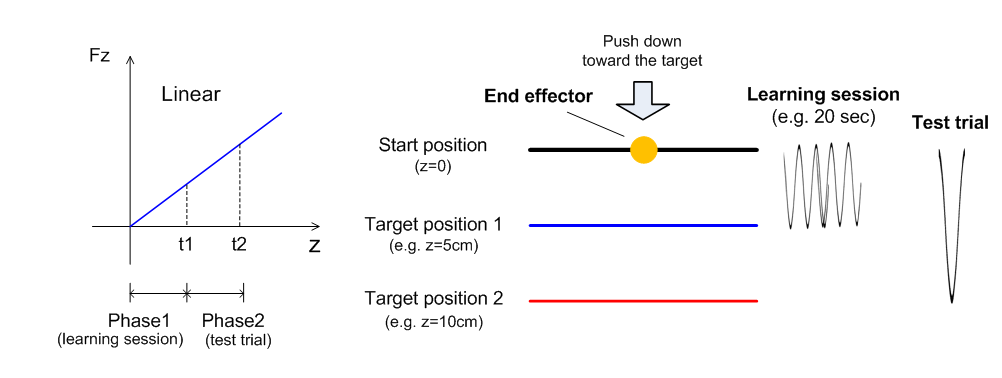
\includegraphics[scale=0.4]{Chie/figs/fig2.png}
  \caption{Experimental Design. Two target positions were set: z = t1
   for learning session and z = t2 for test trial.}
  \label{design}
\end{figure}


\subsection{Apparatus and Stimuli}

The haptic device, ``Haptic Master'' consisted of a large robotic rod with an
end-effector. The ``Home'' position, where was the centre of the end effector
is z = 0 at the workspace, was 110 cm from the ground. The spring position was
set at z = 0. In this study, the rod movements were restricted in the vertical
direction only.

The visual information about the task was provided at the computer display to
human subjects. The computer screen was located at the right side of the
Haptic Master from the subjects; where the centre of the screen was
approximately 80 cm from the centre of the robotic rod. The screen was
approximately 1 m away from the participants' standpoint, and 80 cm away from
the centre of the end effector position. The screen displayed the target
position and the end-effector position in real-time (Fig. 3). The target
positions were set at z = t1 (50 mm for learning), and z = t2 (100 mm for
test).
%
\begin{figure}
  \centering
  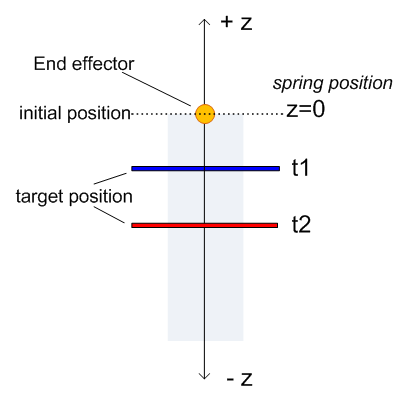
\includegraphics[scale=0.4]{Chie/figs/fig3.png}
  \caption{Experimental visual stimuli. The end-effector and the two target 
   positions (z = t1 and z = t2) were visually indicated on the computer 
   screen.}
  \label{stimuli}
\end{figure}


\subsection{Procedure and analyses}

Participants stood in front of the haptic device and grasped the end-effector. 
Firstly, they conducted a practice session followed by the main blocks. They 
were required to make repetitive movements against compliant force generated by 
the device to learn the kinetic principle. The movements were monitored by 
visual information on the screen. Participants pushed the end-effector to reach 
the target position, and then released the end-effector to allow it to freely 
return to the initial position (z=0). They were asked to set the centre of the 
end-effector position on the target as accurate as possible. 

The main block consisted of two parts: Learning session and Test trial. In the 
Learning session, the target position was set at z= t1, described above. 
Participants controlled the end-effector by their own timing, or rhythm, per 
each movement in the current pilot study (the specific time windows were not 
set up by the programme for the series of movements: i.e., push the 
end-effector down from the start position and reach the target position). 
The visual feedback was given when the end-effector reached to the target; 
the target colour indicated this by changing from blue to yellow. 
Participants learnt the compliant force dynamics by the repetitive movements. 
he experimenter monitored the elapsed time using a stopwatch, and verbally 
informed the end of the session when 20 seconds passed. Participant stopped 
their repetitive movements immediately and prepared for the trial session. 

In the Test trial, participants moved the end-effector to the target (coloured 
red line, z = t2) three times based on the formula they previously learned. In 
this phase, no visual feedback in the relationship between the end-effector 
position and the target was given to the subjects.

One block consists of three sets (Learning session + Test trial). Participants 
conducted three blocks; so, 3 blocks in total, and 9 test trials. Under the 
current settings, the experiment was completed within approximately 20 minutes 
on average.

The dynamic properties of the point-to-point movements were measured: the
end-effector's position ($\BZ$), the velocity ($\dot{\BZ}$), and the force
($\BF_Z$) across the time. These were recorded by the 20 msec sampling rate
 %and the
properties were analysed and compared between the linear and the non-linear
force conditions.

%%%%%%%%%%%%%%%%%%%%%%%%%%%%%%%%%%%%%%%%%%%%%%%%%%%%%%%%%%%%%%%%%%%%%%%%%%%%%%%%
\section{Results and Discussions}

\subsection{Participants}

Six male subjects (age: 28.8 +/- 3.1 (SD), height: 175.3 cm +/- 7.1 (SD), 
weight: 79.5 kg +/- 17.8 (SD), one left-handed) voluntarily participated in the 
pilot experiment. All had normal or corrected to normal vision, and they had no 
known motor deficits and/or any limb injuries (self-reported). They were 
recruited from the student and staff population at University of Birmingham. 
(One was not na�ve to the purpose of the experiment.)


\subsection{Ongoing Results}

The end-effector position, velocity and force were recorded. Here, illustrates
the one participant's one block performance, as an example (Fig 4).

In order to examine the each reaching movement, the data were extracted from 
the total between the start (z = 0.01m) and the end (approx. z = t2) positions, 
where the end-effector was released to return to the initial position. These 
points were determined by calculating the each inflection point (Fig 5).

The data were averaged across three blocks; one block consisted of three
(Learning + Trial) sessions; so participants ideally completed 9 sessions in
total, but one (subj.03) accidentally completed only two blocks because of the
setting errors. The averaged numbers of repetitions were 152.8 +/- 45.6 (SD)
in the Learning session and 27.2 +/- 6.1 (SD) in the Test trial. All six
participants' averaged data (the end-effector position, velocity and force)
can be seen from Fig.6 to Fig. 8.
%
\begin{figure}
  \centering
  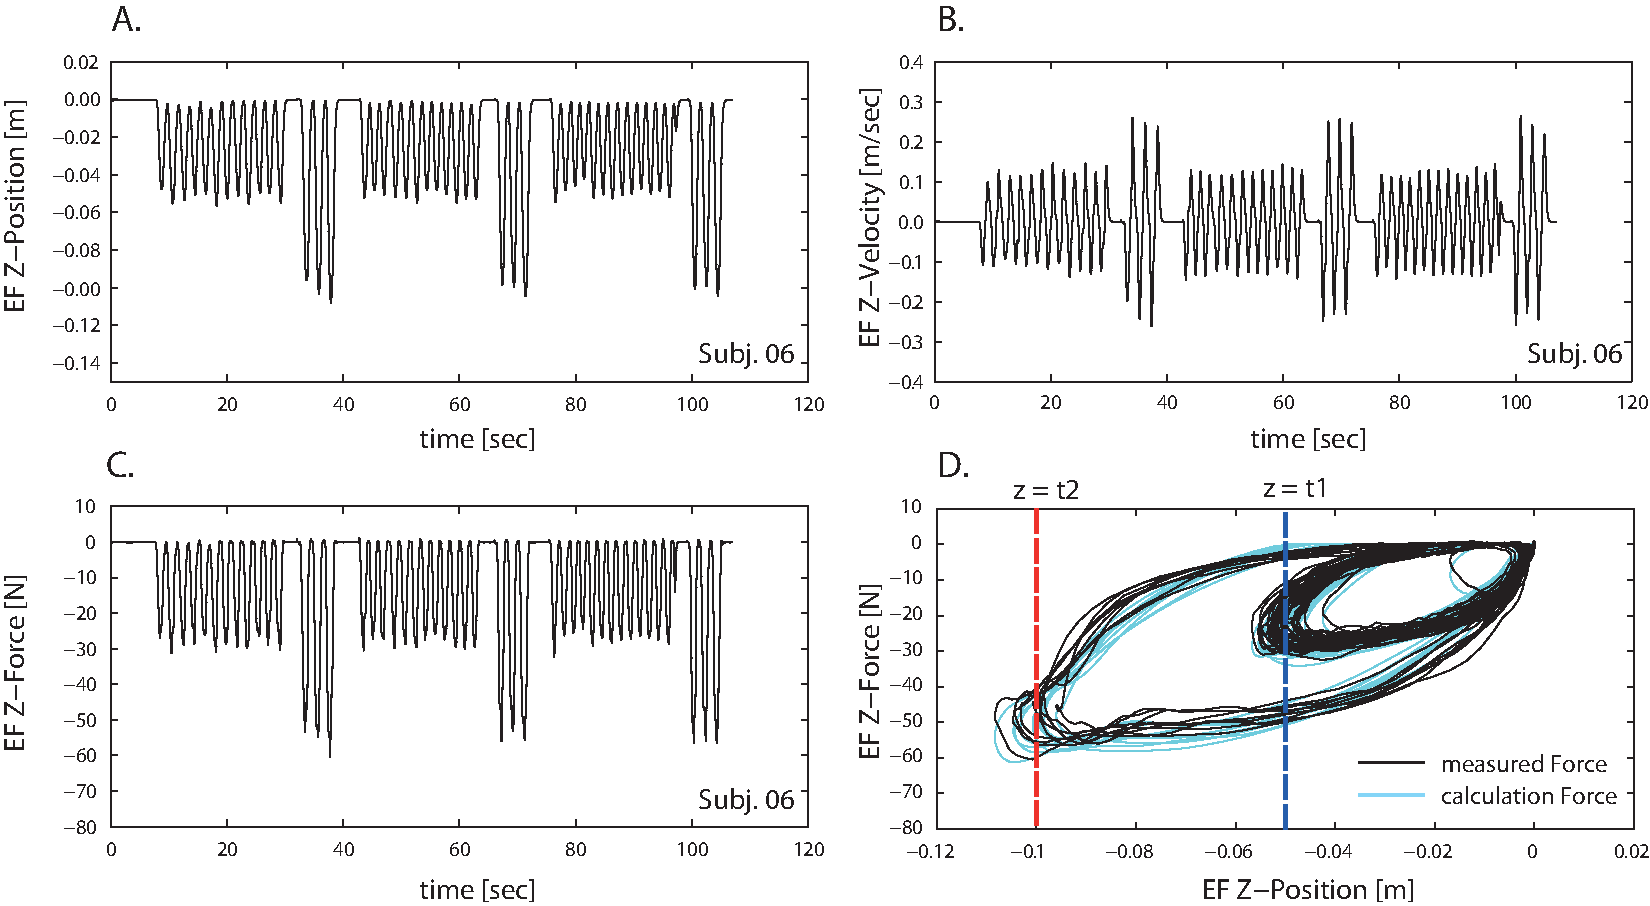
\includegraphics[scale=0.55]{Chie/figs/fig4.pdf}
  \caption{The total recording of the completion of the first block.
    (Subj. 06). $\BA$. End-effector Z-position, $\BB$. Z-velocity and
    $\BC$. Z-force.  $\BD$. the relationship between the position and the
    force compared between the force directly measured by the sensor and the
    force calculated by the equation with the real time z-position and
    z-velocity.}
  \label{results}
\end{figure}
%
\begin{figure}
  \centering
  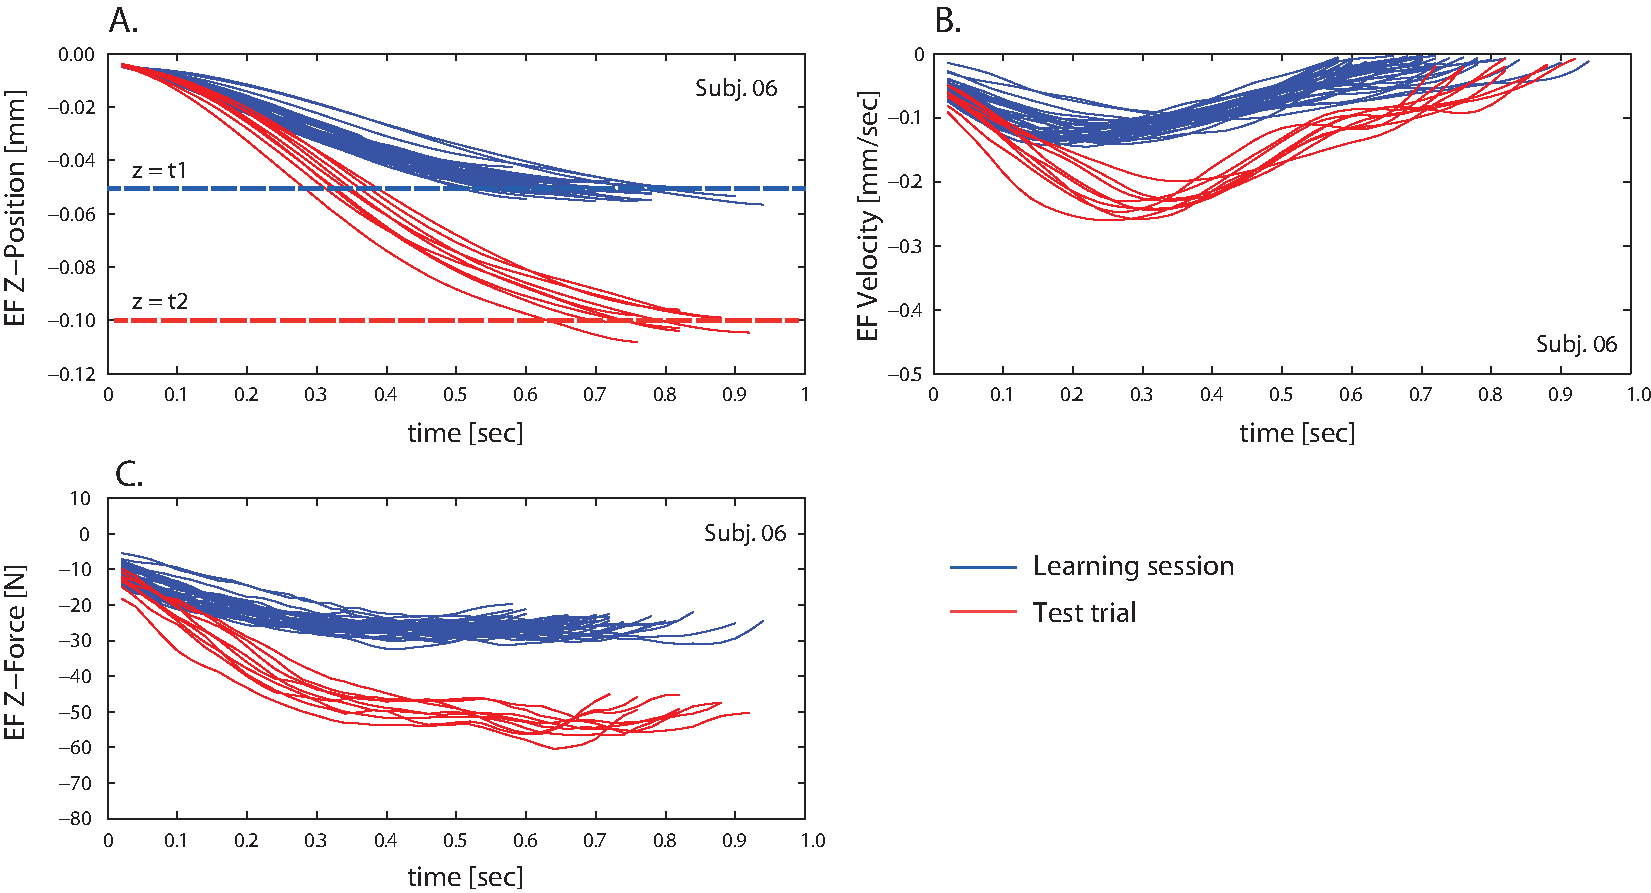
\includegraphics[scale=0.55]{Chie/figs/fig5.pdf}
  \caption{Experimental data for one participant (the first block, three test 
   trials). Red lines represent the forces, which were directly measured by a 
   sensor at the end-effector. Blue lines represent the forces, which were 
   calculated in the real time by spring stiffness and damping factor with 
   the end-effector position.}
  \label{results}
\end{figure}
%
\begin{figure}
  \centering
  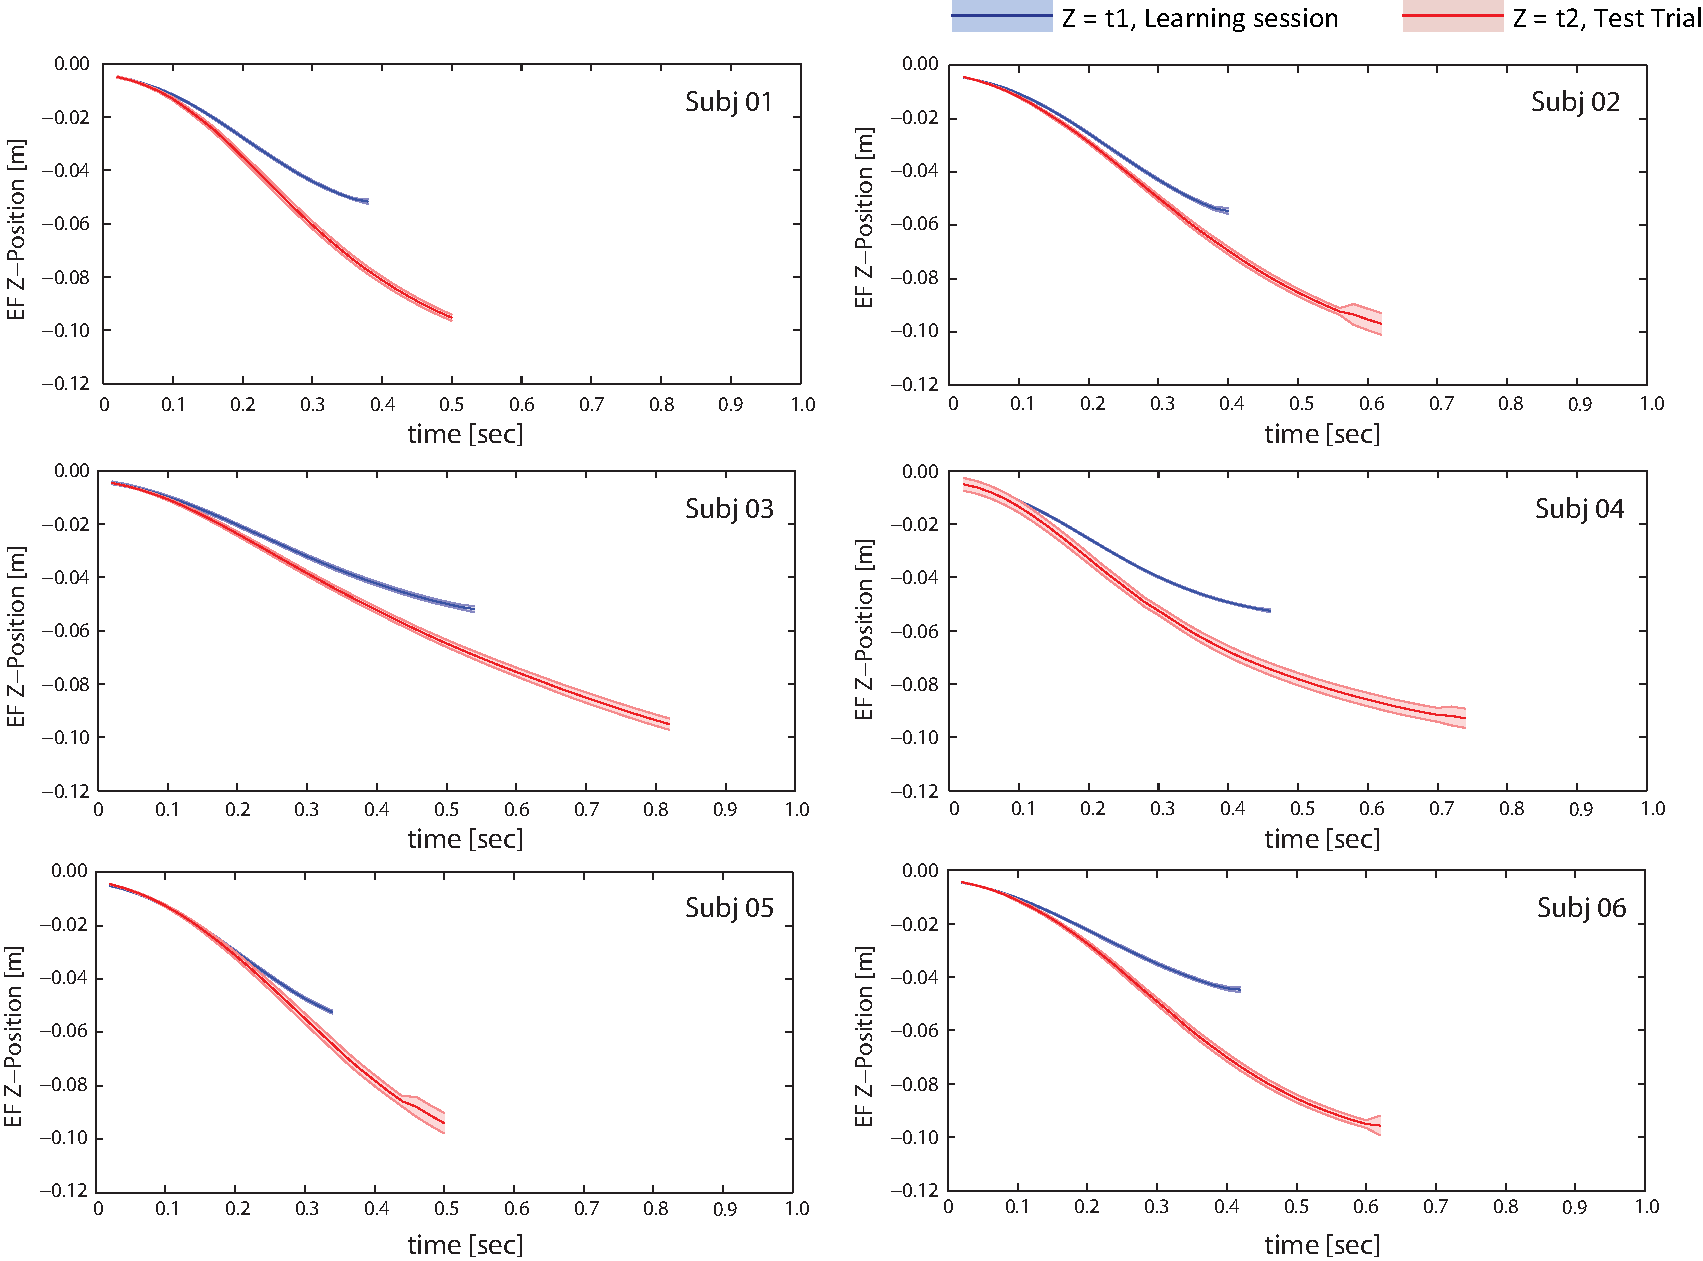
\includegraphics[scale=0.55]{Chie/figs/fig6.pdf}
  \caption{The averaged end-effector z-position performance in the reaching 
   movements against the linear spring-damper force for 6 subjects. 
   The data were averaged across 3 blocks (9 (Learning + Trial) sessions). 
   The blue lines represent the average performance in the Learning session, 
   and the red in the Test trial, the coloured areas represent their standard 
   error respectively.}
  \label{results}
\end{figure}

\begin{figure}
  \centering
  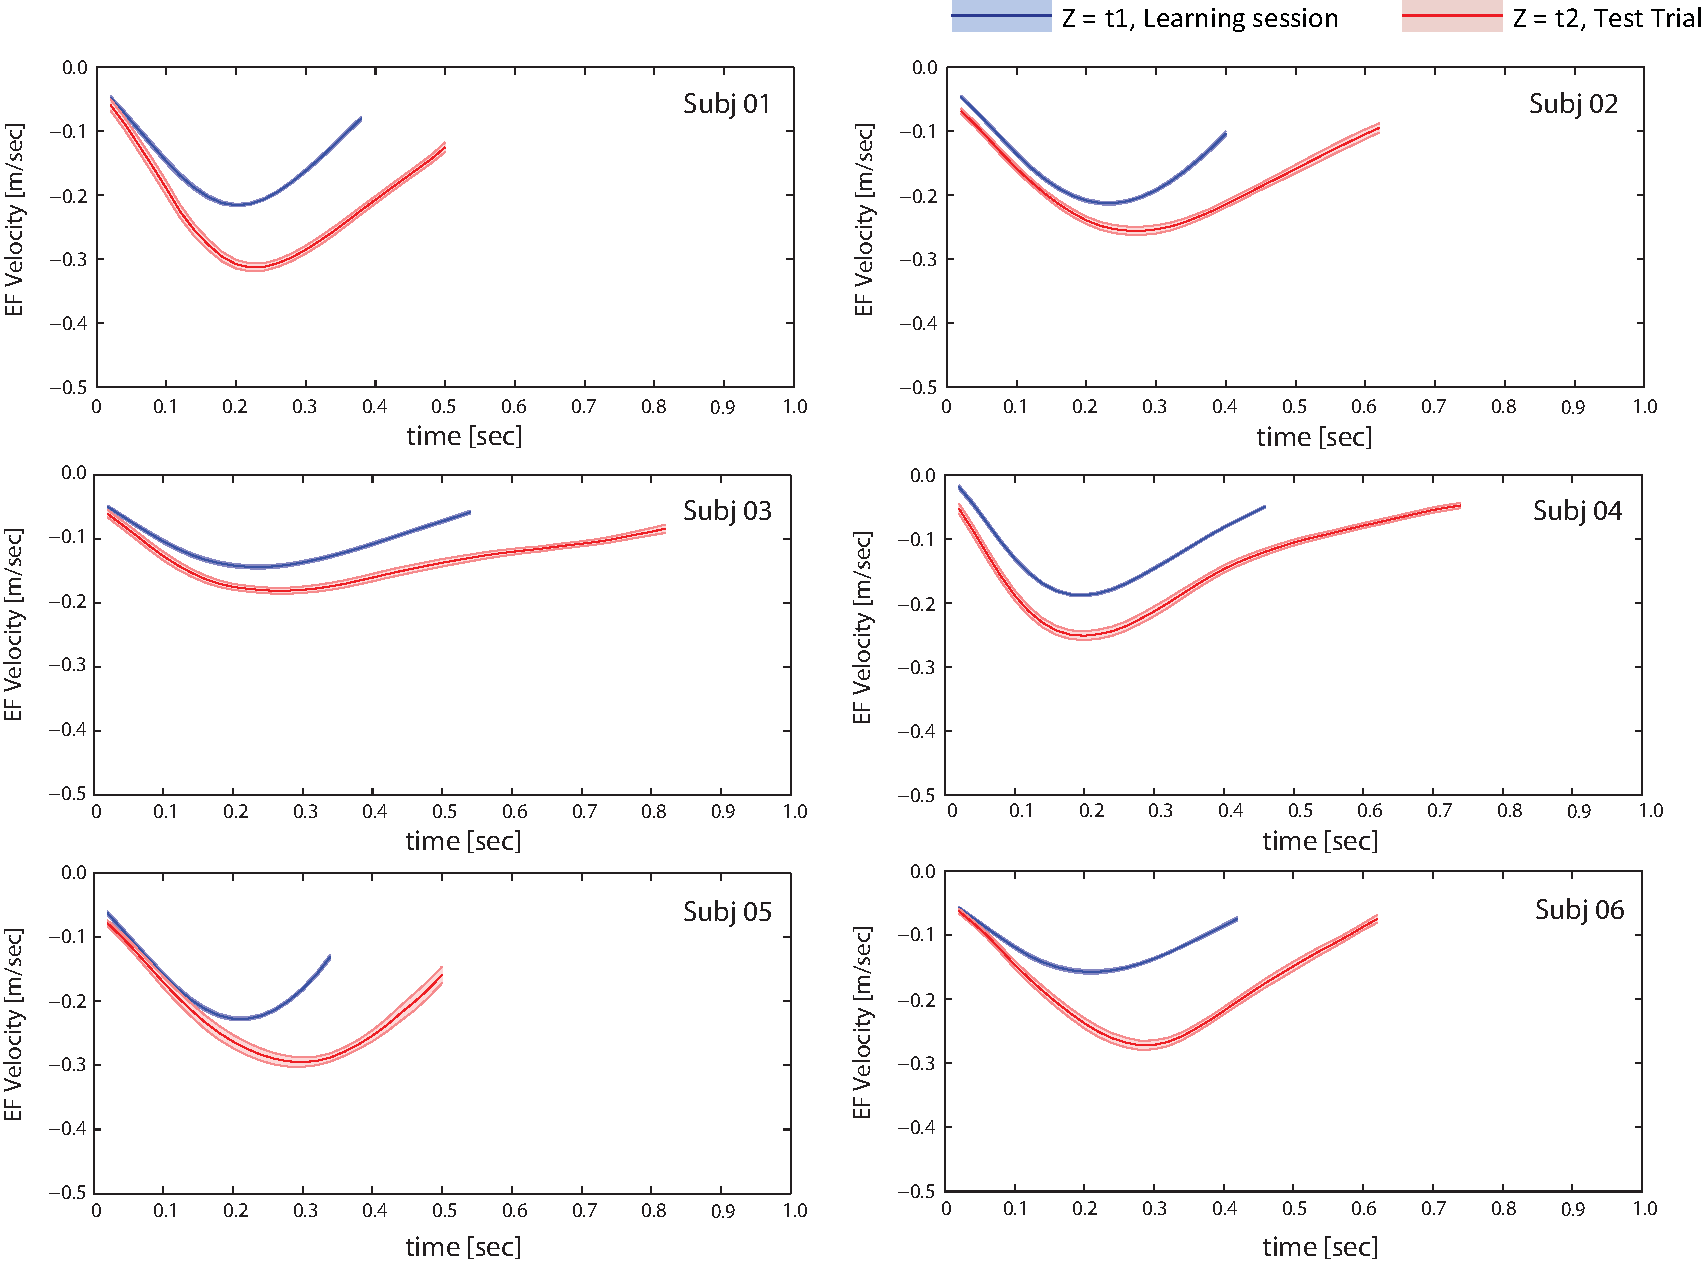
\includegraphics[scale=0.55]{Chie/figs/fig7.pdf}
  \caption{The averaged end-effector z-velocity performance in the reaching 
   movements against the linear spring-damper force for 6 subjects. 
   The data were averaged across 3 blocks (9 (Learning + Trial) sessions). 
   The blue lines represent the average performance in the Learning session, 
   and the red in the Test trial, the coloured areas represent their standard 
   error respectively.}
  \label{results}
\end{figure}

\begin{figure}
  \centering
  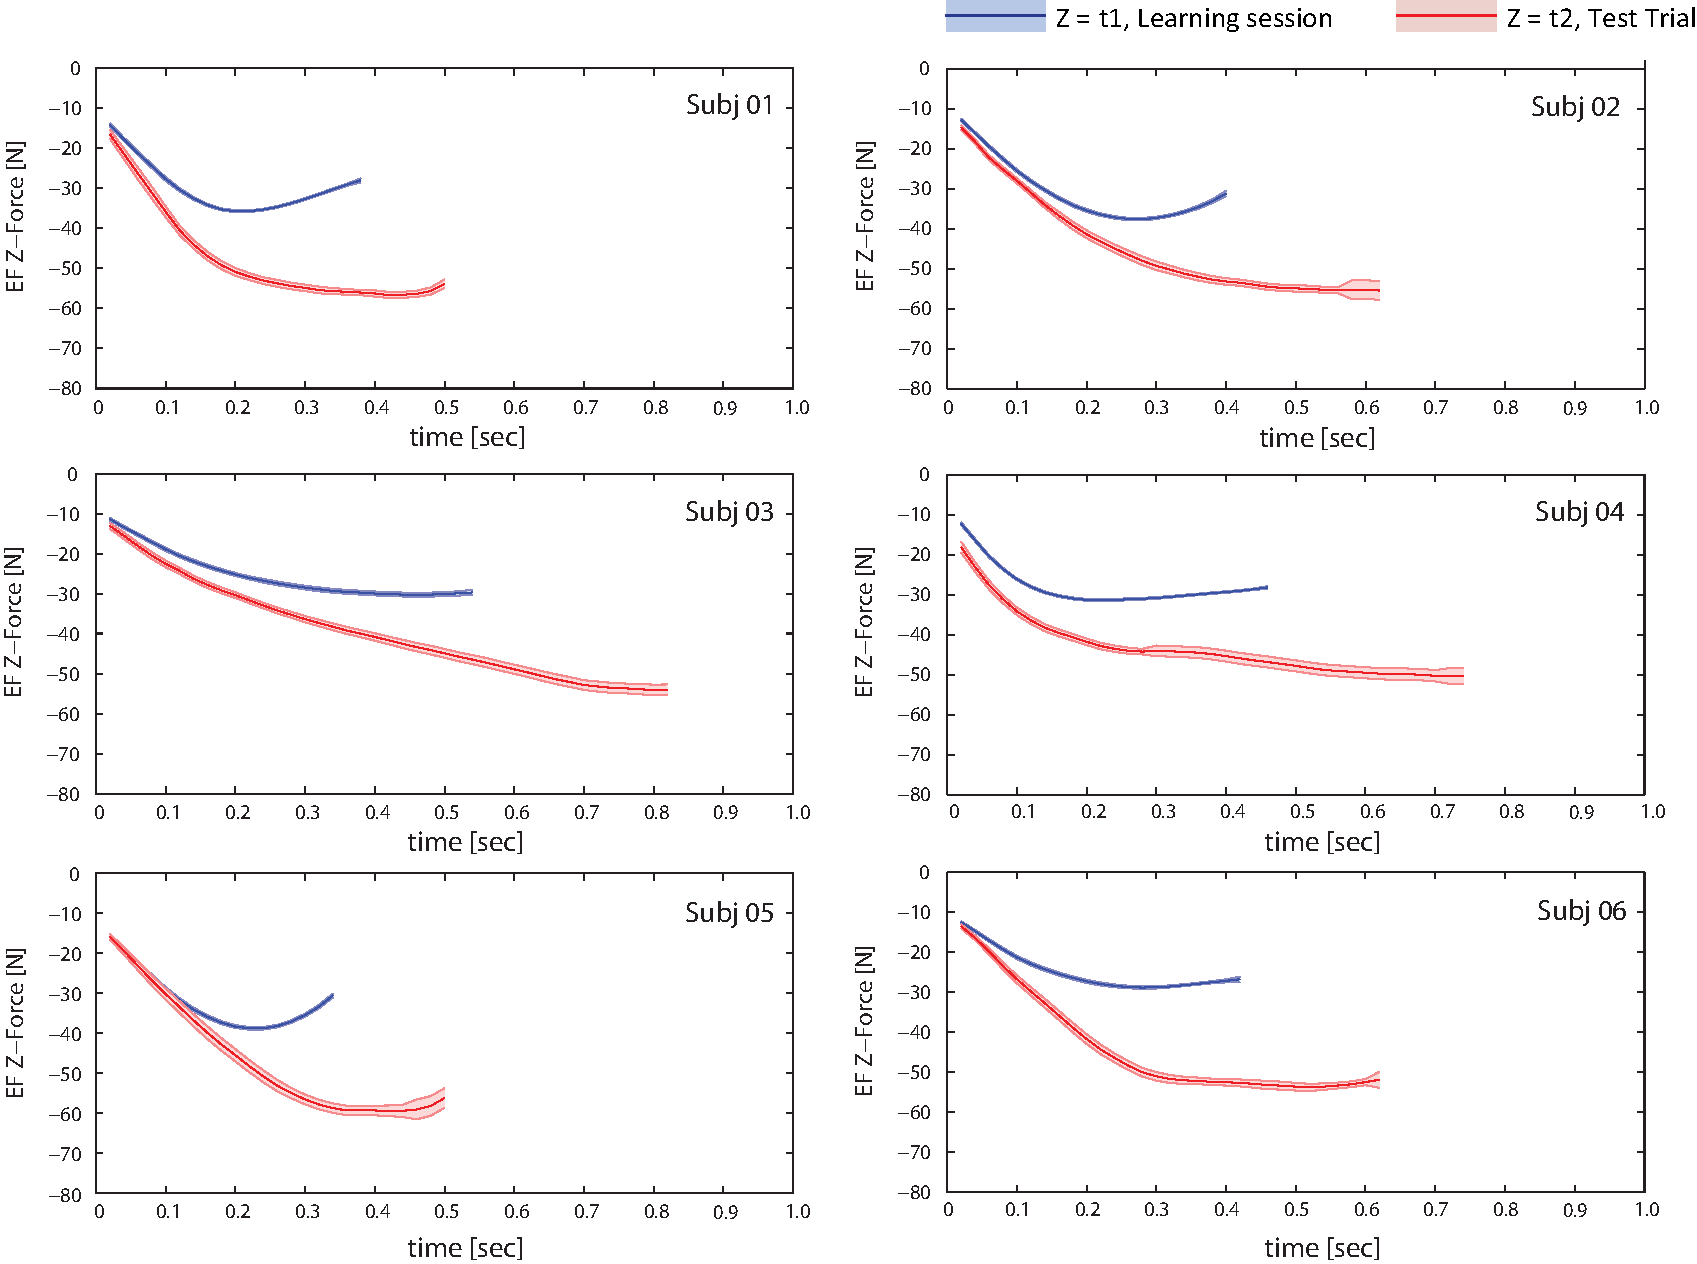
\includegraphics[scale=0.55]{Chie/figs/fig8.pdf}
  \caption{The averaged end-effector z-force performance in the reaching 
   movements against the linear spring-damper force for 6 subjects. 
   The data were averaged across 3 blocks (9 (Learning + Trial) sessions). 
   The blue lines represent the average performance in the Learning session, 
   and the red in the Test trial, the coloured areas represent their standard 
   error respectively.}
  \label{results}
\end{figure}

\begin{figure}
  \centering
  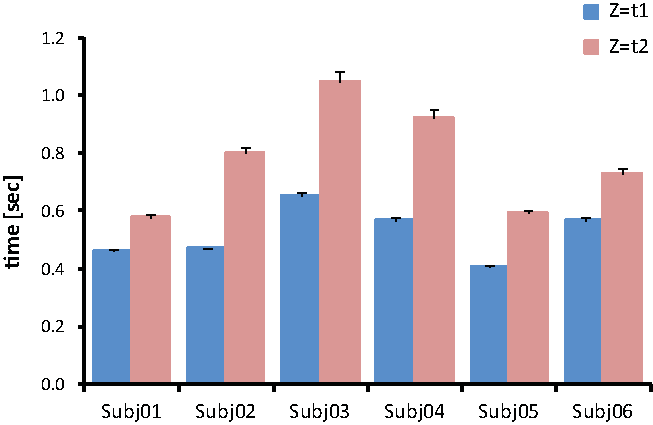
\includegraphics[scale=1]{Chie/figs/fig9.pdf}
  \caption{Illustrate averaged time to reach the targets with the comparison 
   between the Learning session (blue) and the Test trial (red) for six 
   subjects. The error bars represents the standard error across the total 
   number of the repetitions.}
  \label{results}
\end{figure}


\subsection{Brief Discussion}

The Fig 9 showed that some participants (e.g., Subj.01, Subj.06) performed to 
reach the target position (z = t2) much faster than the expected time duration, 
which was estimated from the linear equation. That is, the t2 position was 
double distance of the t1 from the start position; so the reaching time would 
be estimated close to the double. The time would not be able to calculate by 
the simple linear calculation because the damping factor depends on the 
velocity, though.

This might be caused by the experimental design; that is, participants made
the repetitive movements with their own rhythms at the learning
session. Because they tend to keep their rhythms even in the consecutive trial
session, and then they might have unconsciously increased the force or
accelerated their speed to reach the target. This possibility can be seen at
their movement profiles (Fig.7: velocity and Fig.8: force). Several studies
have shown that time perception plays an important role in human motor control
\cite{Berret&Jean16, Rank&DiLuca15}; therefore, this timing issue should be
carefully considered into the experimental design and should avoid any
confounding factors. To do this, we will visually guide the participants'
movements with a certain time-windows in the future experiment.

Moreover, in the current pilot experiment, the judgment of reaching the target
was inaccurate. Although the participants received the visual feedback at the
learning session, it only indicated the end-effector crossed the target
position, and also there were no task reward. The inaccuracy would have
affected their force perception and movements \cite{Rank&DiLuca15} therefore,
in the next experiment, we will set a specific correct zone visually defined
by a more accurate way (e.g. the similar size of sphere of the end-effector)
as the target instead of the line indicators. The task completion in the
Learning session would be determined by their performance and individual
learning level would be evaluated by their correct movements.

The current analyses conducted for all performance in the test trial (reaching 
the target (z= t2) three times for each), but the performance might have needed 
to be evaluated focusing on the first trial only, because the first movement 
was directly affected by the learning session and the second and the third 
movements were gradually contaminated.

Overall, through the pilot experiment, we have learned the importance of the 
timing issue in interacting with compliant surface. We will improve the 
experimental design and strictly control the parameters (timing, speed, 
and the accuracy). 

In the future experiment, based on the linear case, we will measure the 
pattern under the non-linear compliant forces and examine the human 
goal-directed performance. Besides, as well as the spring-damper, it may 
help the understanding of the generalization if we employ another compliant 
force model (e.g. object surface).
